\chapter{Evaluation and results}
\nomenclature[A]{RMSE}{Root Mean Square Error}

To evaluate the performance of the proposed wind estimation algorithm and the wind compensation strategies, a simulation-based test framework is established. 
For the wind estimation task, the performance of the Extended Kalman Filter (EKF) and Unscented Kalman Filter (UKF) is compared under identical conditions. For wind compensation, Disturbance Feedforward (DFF) and Nonlinear Dynamic Inversion (NDI) are evaluated with respect to their impact on tracking performance and compared to the baseline PID controller.

To ensure a representative evaluation under different operating conditions, six flight scenarios are considered. These flight scenarios reflect the main real-world operational scenarios.

\begin{itemize}
	\item Forward flight: slow (\SI{2}{m/s}) and fast ($4~\mathrm{m/s}$)
	\item Sideward flight ($1~\mathrm{m/s}$)
	\item Pure rotation around the yaw axis ($5^\circ/\mathrm{s}$)
	\item Curved flight: forward flight (($1~\mathrm{m/s}$) combined with a yaw rotation ($3.6^\circ/\mathrm{s}$)
	\item Hover
\end{itemize}

Since the performance of the wind estimation and compensation methods depends strongly on the wind conditions, multiple wind scenarios are considered for each flight scenario. These include different constant wind velocities and varying turbulence intensities generated by varying the Dryden model parameter $W_{20}$, as introduced in Section~\ref{sec:2.3WindModel}.

The root mean square error (RMSE) is used as the primary performance metric throughout this evaluation. It provides a quantitative measure of the deviation between a reference signal and its corresponding estimate or response. For a signal $x$ with $N$ samples, the RMSE is defined as \cite{Chai2014RMSE}

\begin{equation}
	\mathrm{RMSE}(x) =
	\sqrt{
		\frac{1}{N}
		\sum_{k=1}^{N}
		\left(x_k-\hat{x}_k\right)^2
	},
	\label{eq:rmse}
\end{equation}

where $x_k$ denotes the reference value and $\hat{x}_k$ the corresponding estimated or simulated value at sample $k$.

In the following evaluation, the RMSE is applied to assess both the wind estimation accuracy and the resulting state tracking performance. The wind RMSE quantifies the deviation between the estimated and actual wind components, while the state RMSE is used to evaluate the tracking error of the airship states. 

Include average RMSE. (within the same category pos, vel, ... an average RMSE can be meaningful and is used throughout this thesis. (Find citation))

The remainder of this chapter is structured as follows. In Section~\ref{sec:5.1WindEstimation}, the performance of the wind estimation algorithm is evaluated for the considered flight and wind scenarios. Subsequently, Section~\ref{sec:5.2WindCompensation} investigates the effectiveness of the proposed wind compensation strategies and their impact on the overall control performance.

\section{Wind estimation}
\label{sec:5.1WindEstimation}

Following the wind estimation performance is analyzed. To use our Dryden model, which is interconnected to our airship model, we first need to specify its parameters, especially W20 as the rest is all state dependent.
First of all we need to find a W20 parameter. We choose W20 = 5, which is justified in the section \todo{ref}.

Result: Good wind estimation....
yields a good basis for wind compensation where good disturbance estimation is one requirement.





\subsection{Sensitivity to wind parameters}
\label{sec:5.1.1W20}

As stated in introduction wind the parameter reference wind velocity W20 cannot be determined depending on states directly, it has to be estimated beforehand. We cannot know the true W20 value of the environment, but we have to give it to the wind model incorporated into the model. So we need to find an estimate for W20 that works with all wind scenarios we encounter and want to achieve good performance for (up to 30kmh) 

The wind parameters W20 and wind direction cannot be measured or computed directly from the states and thus need to be estimated. In the following the sensitivity to the correct parameter is assessed.
Therefore multiple tests are carried out. 

First a constant parameter value for W20 was specified, creating the actual wind turbulences in the simulation. The wind estimation performance was assessed for varying estimated W20, reaching from W20 = 0 up to W20 = 30 km/h. For each estimated W20 parameter value 27 wind scenarios are run. In each wind scenario the constant wind, as well as the random seed creating the turbulences, were varied resulting in unique wind conditions for each test.
For each test the RMSE between the estimated wind and actual wind are computed individually and the average RMSE along all three axis is computed.
Then the results are averaged among all 27 wind scenarios.
The results are shown in Table \ref{fig:W20_Barchart} and lead to the following conclusions. 

% W20 comparision plot
\begin{figure}[htbp]
	
	\centering
	
	\definecolor{barblue}{RGB}{55,138,221}
	\definecolor{barmatch}{RGB}{216,90,48}
	
	\pgfplotsset{
		rmse bar/.style={
			ybar,
			bar width=14pt,
			width=\textwidth,
			height=5cm,
			enlarge x limits=0.1,
			xlabel={$W20_{\text{est}}$},
			ylabel={RMSE Total},
			ymin=0,
			ymax=1.6,
			xtick={0,1,2,3,4,5,6,7},
			xticklabels={0, 1.6, 3.3, 5, 6.6, 8.3, 10, 15},
			xticklabel style={font=\small},
			yticklabel style={font=\small},
			xlabel style={font=\small},
			ylabel style={font=\small},
			ymajorgrids=true,
			bar shift=0pt,
			grid style={gray!20}
		}
	}
	
	% ----- W20_est = 0  (match at index 0) -----
	\begin{subfigure}[b]{0.48\textwidth}
		\centering
		\begin{tikzpicture}
			\begin{axis}[rmse bar, title={$W20_{\text{act}}=0$}]
				% all bars blue
				\addplot[fill=barblue] coordinates {
					(0,0.8889)(1,0.2964)(2,0.2599)(3,0.2193)(4,0.2487)(5,0.2388)(6,0.2338)(7,0.2227)
				};
				% overdraw match bar in orange
				\addplot[fill=barmatch] coordinates { (0,0.8889) };
			\end{axis}
		\end{tikzpicture}
	\end{subfigure}
	\hfill
	% ----- W20_est = 1.6  (match at index 1) -----
	\begin{subfigure}[t]{0.48\textwidth}
		\centering
		\begin{tikzpicture}
			\begin{axis}[rmse bar, title={$W20_{\text{act}}=1.6$}]
				\addplot[fill=barblue] coordinates {
					(0,0.9617)(1,0.3323)(2,0.2663)(3,0.2357)(4,0.2585)(5,0.2519)(6,0.2479)(7,0.2434)
				};
				\addplot[fill=barmatch] coordinates { (1,0.3323) };
			\end{axis}
		\end{tikzpicture}
	\end{subfigure}
	
	\vspace{1em}
	
	% ----- W20_est = 5  (match at index 3) -----
	\begin{subfigure}[t]{0.48\textwidth}
		\centering
		\begin{tikzpicture}
			\begin{axis}[rmse bar, title={$W20_{\text{act}}=5$}]
				\addplot[fill=barblue] coordinates {
					(0,1.2059)(1,0.5220)(2,0.4277)(3,0.3801)(4,0.3966)(5,0.3868)(6,0.3716)(7,0.3662)
				};
				\addplot[fill=barmatch] coordinates { (3,0.3801) };
			\end{axis}
		\end{tikzpicture}
	\end{subfigure}
	\hfill
	% ----- W20_est = 8.3  (match at index 5) -----
	\begin{subfigure}[t]{0.48\textwidth}
		\centering
		\begin{tikzpicture}
			\begin{axis}[rmse bar, title={$W20_{\text{act}}=8.3$}]
				\addplot[fill=barblue] coordinates {
					(0,1.4843)(1,0.8910)(2,0.7633)(3,0.7158)(4,0.7111)(5,0.6595)(6,0.6362)(7,0.6059)
				};
				\addplot[fill=barmatch] coordinates { (5,0.6595) };
			\end{axis}
		\end{tikzpicture}
	\end{subfigure}
	
	\caption{Comparison of Total RMSE Across All Estimated $W20$ Wind Speeds. The orange bar highlights the true configuration scenario where $W20_{\text{est}} = W20_{\text{act}}$.}
	\label{fig:W20_Barchart}
\end{figure}

a) Even for constant wind $W20_{\text{act}} = 0$, an estimate of $W20_{\text{est}} = 0$ leads to bad results. This can be explained when looking at the computation of the Wind Process noise, for $W20_{\text{est}} = 0$, this results in qwind = 0 \todo{proof}, thus not allowing the wind estimate to change at all. So the initial guess will be kept forever? \todo{really? or just for constant wind = 0} deviation, due to the nonperfect modelling and uncertainties in place. (For perfect modelling this deviation would be zero)
b) matching W20 do not always imply best performance. Reason herefore are errors in modelling and bigger W20 more flexibility to adapt.
So why not chosing W20 = 15 for all?
Now look at plots showing differences and oscillations.


The results indicate that a despite the real W20 parameter an estimated W20 = 10 yields good results for all real wind conditions created by varying W20. This can be explained as follows: a bigger W20 estimated increases the Process noise, thus giving the wind states more freedom to react to fast changing wind gusts. This comes at a cost which is a more noisy estimation of the wind. W20 estimated = 10 seems to offer a good tradeoff although bigger values may lead to an even lower RMSE. And bigger W20 leads to bigger qwind, this may have bad side-effects.


\begin{figure}[htbp]
	\centering
	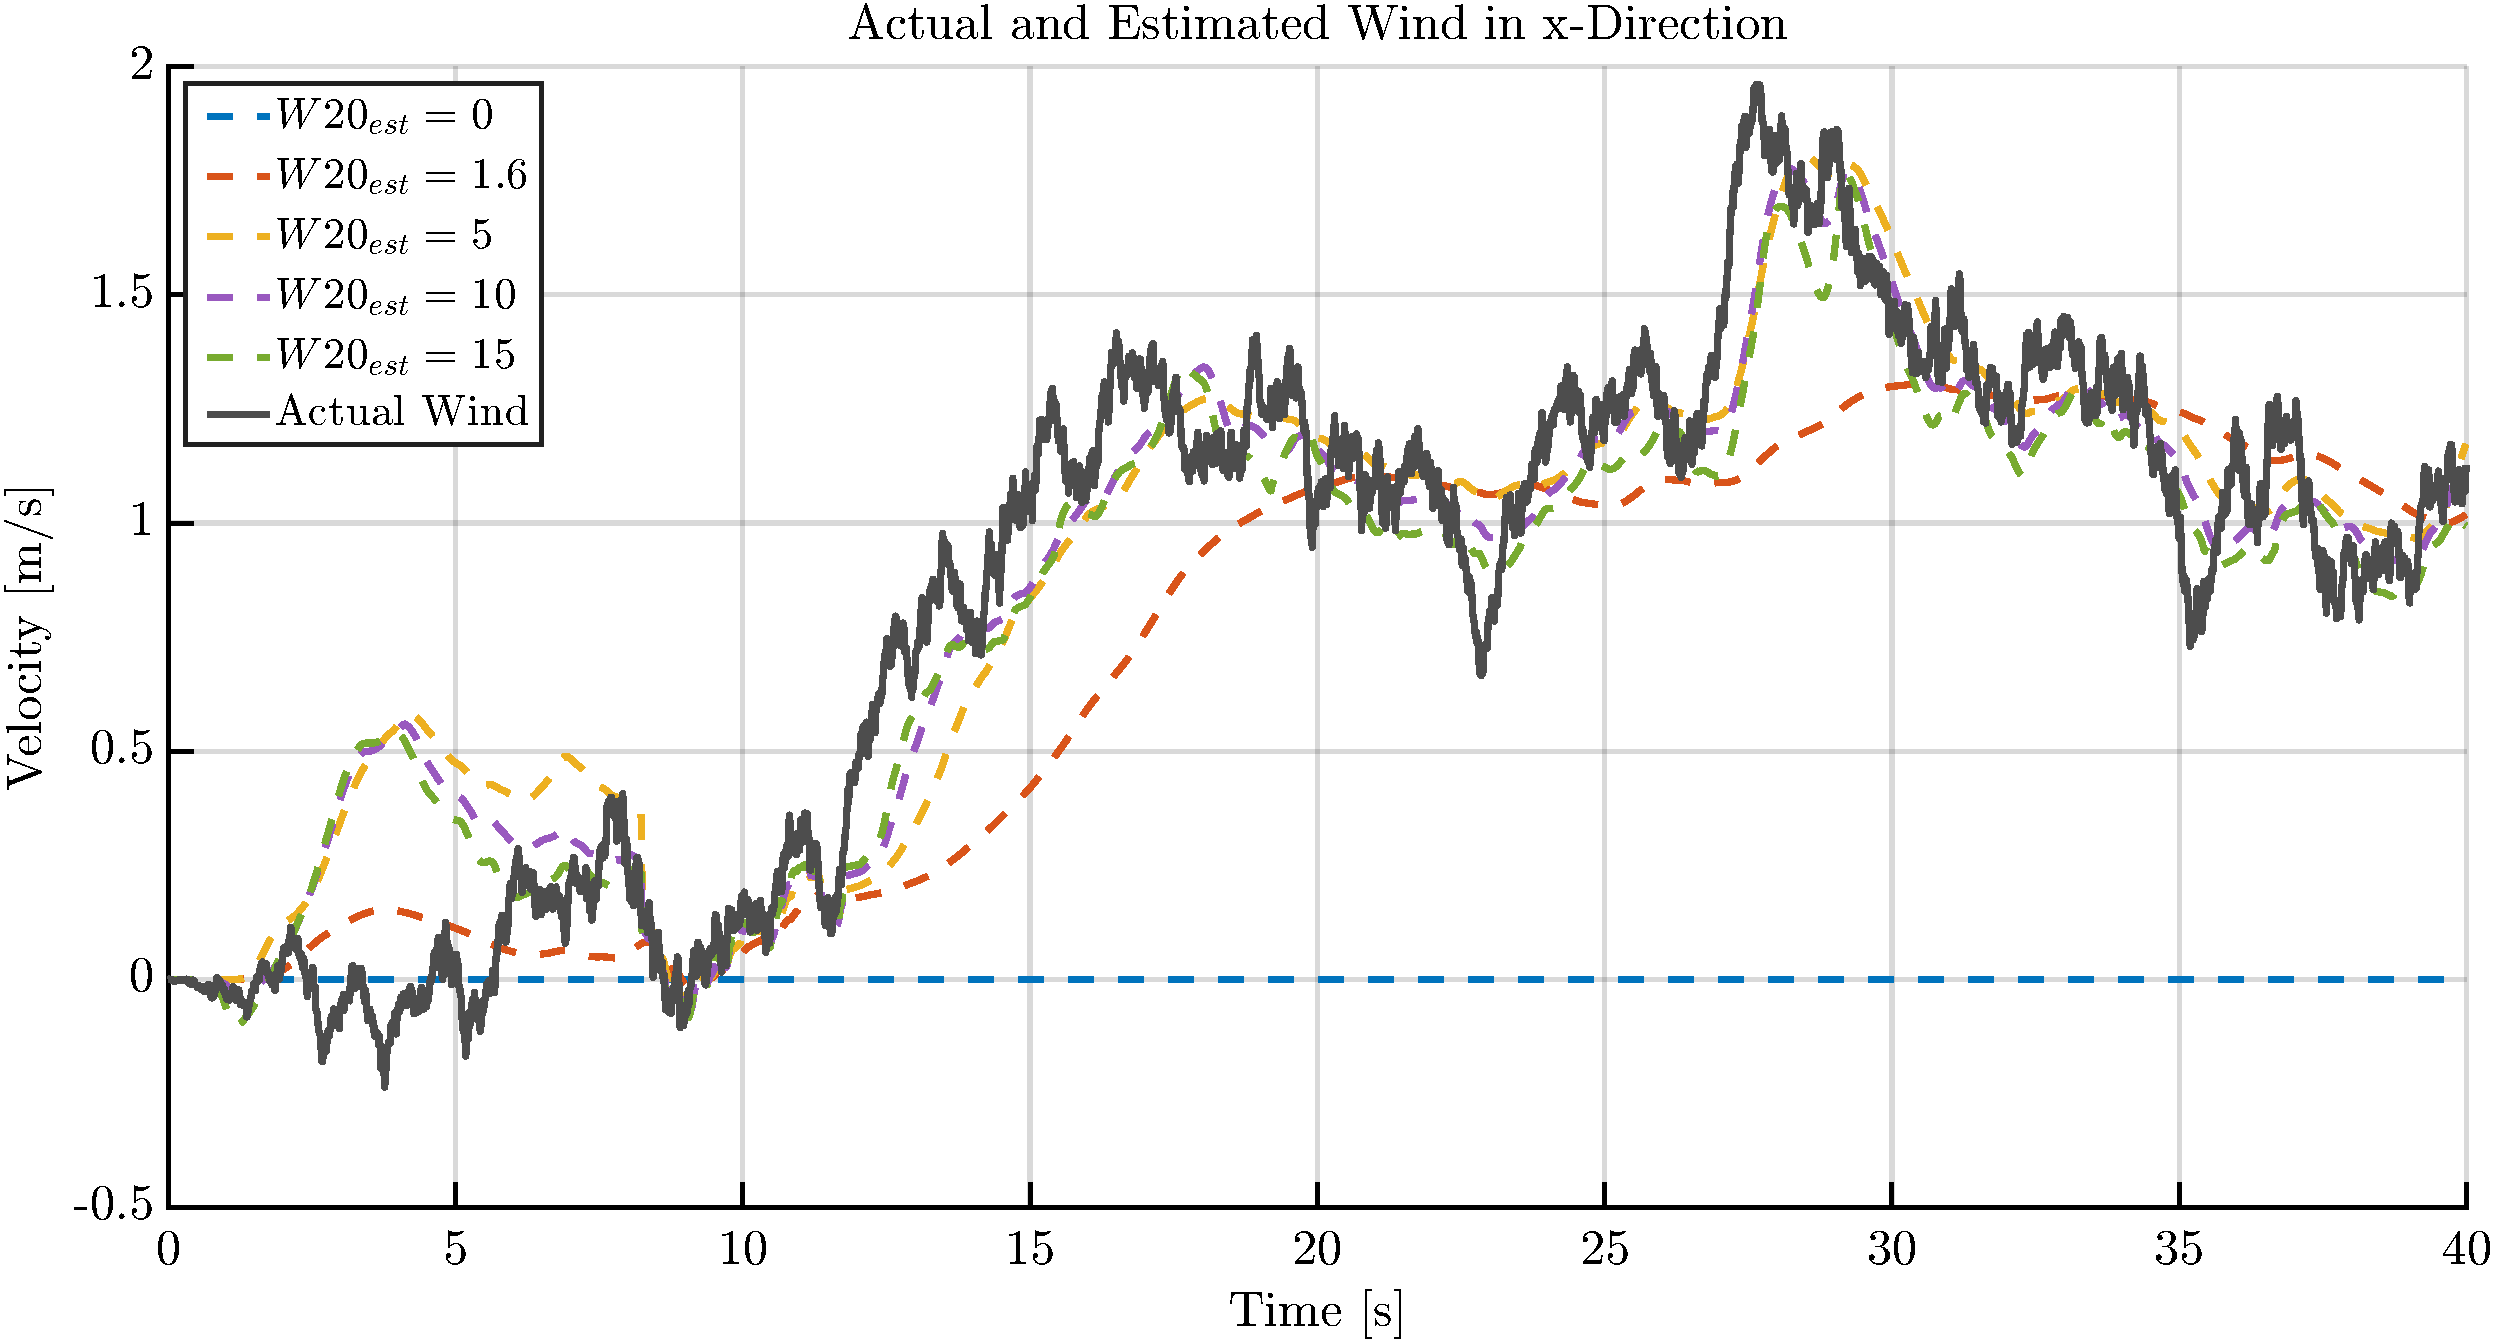
\includegraphics[width=\textwidth]{src/pics/W20_comparision.pdf}
	\caption{Comparision of wind estimation performance for different estimated W20, W20 actual is 5.}
	\label{fig:my_figure}
\end{figure}

What happens with the wind estimation if W20est too big?
-> if theres deviation in the measurements and the expected behaviour computed by the kalman filter, the error will more likely be attributed to the wind as its more uncertain.

%\begin{table}[ht]
%	\centering
%	\begin{tabular}{ccclllll}
%		\toprule
%		$W_{20,\text{est}}$ & $W_{20,\text{act}}$ & Case &
%		$\overline{\text{RMSE}}_{e_1}$ & $\overline{\text{RMSE}}_{e_2}$ &
%		$\overline{\text{RMSE}}_{e_3}$ & $\overline{\text{RMSE}}_{\text{total}}$ \\
%		\midrule
%		\multirow{2}{*}{0.0}   & 0.0  & match & 1.6667 & 0.6667 & 0.3333 & 0.8889 \\
%		& 15.0 & best  & 0.3844 & 0.1603 & 0.1233 & 0.2227 \\
%		\addlinespace
%		\multirow{2}{*}{1.6}   & 1.6  & match & 0.5006 & 0.2634 & 0.2329 & 0.3323 \\
%		& 15.0 & best  & 0.3918 & 0.1885 & 0.1501 & 0.2434 \\
%		\addlinespace
%		\multirow{2}{*}{5.0}   & 5.0  & match & 0.4597 & 0.3414 & 0.3393 & 0.3801 \\
%		& 15.0 & best  & 0.4599 & 0.3292 & 0.3094 & 0.3662 \\
%		\addlinespace
%		\multirow{2}{*}{8.3}   & 8.3  & match & 0.7350 & 0.6243 & 0.6192 & 0.6595 \\
%		& 15.0 & best  & 0.6801 & 0.5593 & 0.5784 & 0.6059 \\
%		\bottomrule
%		
%	\end{tabular}
%		\caption{Mean RMSE of wind estimation error signals per $(W_{20,\text{est}},\, W_{20,\text{act}})$ pair.
%		For each $W_{20,\text{est}}$ the matching case ($W_{20,\text{act}} = W_{20,\text{est}}$)
%		and the case yielding the lowest overall RMSE are shown.}
%	\label{tab:rmse_w20}
%\end{table}





\subsection{UKF vs EKF}

\begin{figure}[htbp]
	\centering
	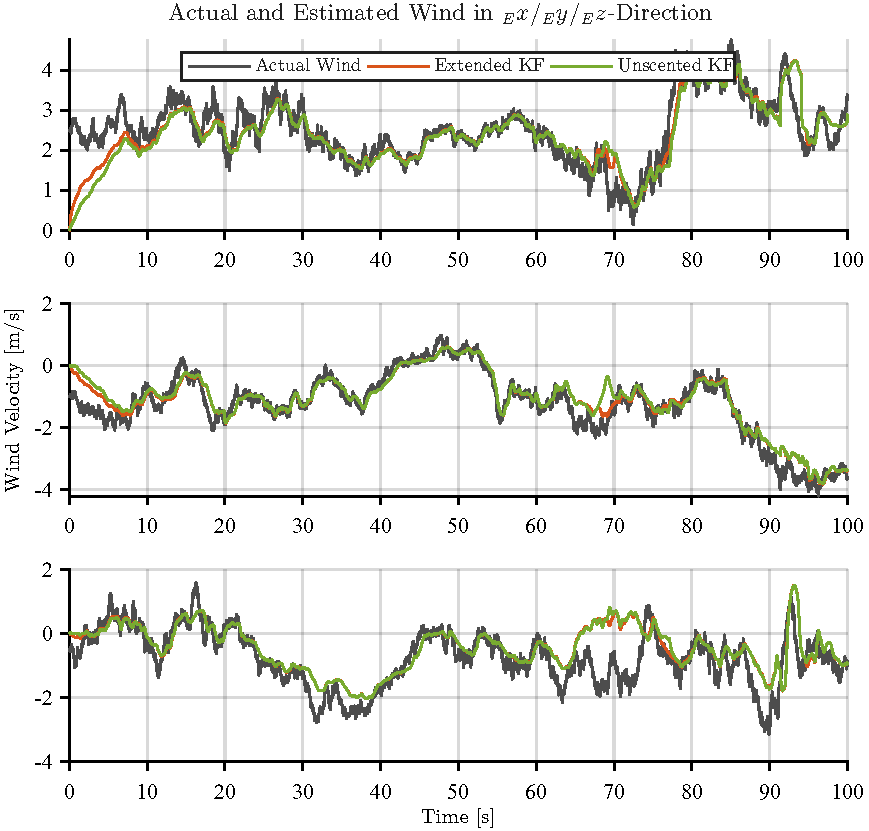
\includegraphics[width=\textwidth]{src/pics/EKFvsUKF_timeplot_curve_10_25_-10_-5.pdf}
	\caption{Comparision of wind estimation performance for different estimated W20, W20 actual is 5.}
	\label{fig:my_figure}
\end{figure}

One can nicely see the transient pahse as described in \ref{sec:3.1.7Initialization}. the init doesnt matter for long term

\begin{figure}[htbp]
	\centering
	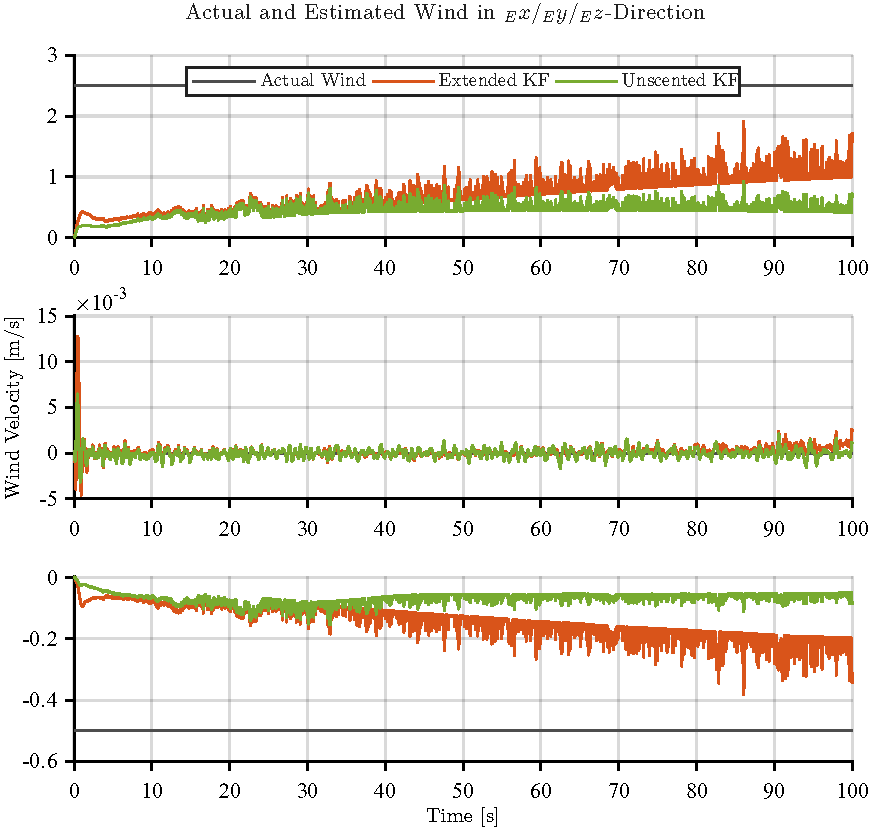
\includegraphics[width=\textwidth]{src/pics/EKFvsUKF_timeplot_hover_0_25_0_-5.pdf}
	\caption{Comparision of wind estimation performance for different estimated W20, W20 actual is 5.}
	\label{fig:my_figure}
\end{figure}


when setting the force uncertainty to zero the oscillations vanish (for R = 0 only convergence rate is improved)
\begin{figure}[htbp]
	\centering
	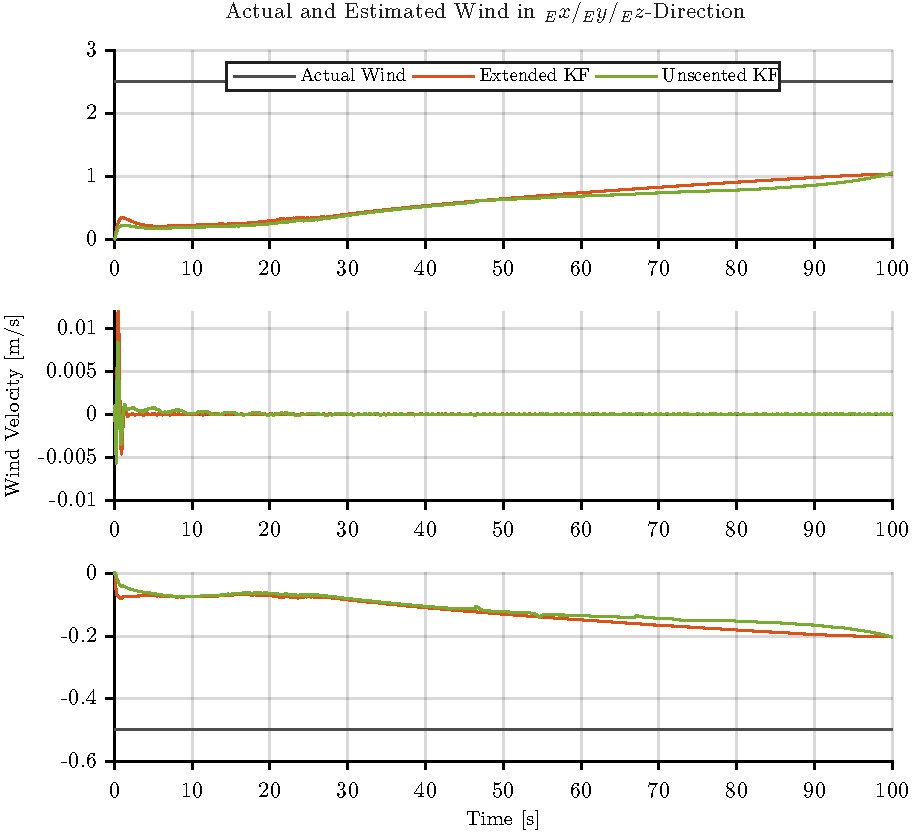
\includegraphics[width=\textwidth]{src/pics/EKFvsUKF_timeplot_hover_0_25_0_-5_no_unc.pdf}
	\caption{Comparision of wind estimation performance for different estimated W20, W20 actual is 5.}
	\label{fig:my_figure}
\end{figure}

Given W20 = 10, 
the rmse is averaged along all three wind directions.

we want to compare the performance of the UKF with that of the EKF. The UKF is fundierter while the EKF is easy to implement on the airship. 

We look at converged data

Goal: Show that performance differs for W20 and flight scenario. Show that EKF and UKF perform almost equally

Therefore a test run was performed:


% -----------------------------------------------------------
% Table: Hover scenario performance by turbulence intensity -
% converged
% -----------------------------------------------------------
\begin{table}[htbp]
	\centering
	\caption{Wind-estimation RMSE for the \textit{hover} scenario by turbulence intensity $W_{20}$, computed on the converged window ($t = 20$--$100\,\mathrm{s}$).}
	\label{tab:hover_w20_conv}
	\begin{tabular}{lrrrrrr}
		\toprule
		& \multicolumn{3}{c}{UKF} & \multicolumn{3}{c}{EKF} \\
		\cmidrule(lr){2-4} \cmidrule(lr){5-7}
		$W_{20}$ & Mean & Std & Median & Mean & Std & Median \\
		\midrule
		0  (none)     & 0.711 & 0.297 & 0.858 & 0.479 & 0.244 & 0.506 \\
		5  (light)    & 0.612 & 0.389 & 0.609 & 0.459 & 0.232 & 0.485 \\
		10 (moderate) & 0.493 & 0.212 & 0.432 & 0.476 & 0.171 & 0.457 \\
		\bottomrule
	\end{tabular}
\end{table}
\todo{include in observability explanaiton}

Yes actually stronger wind helps the estimate this has to do with observability

% Histogram
\begin{figure}[htbp]
	\centering
	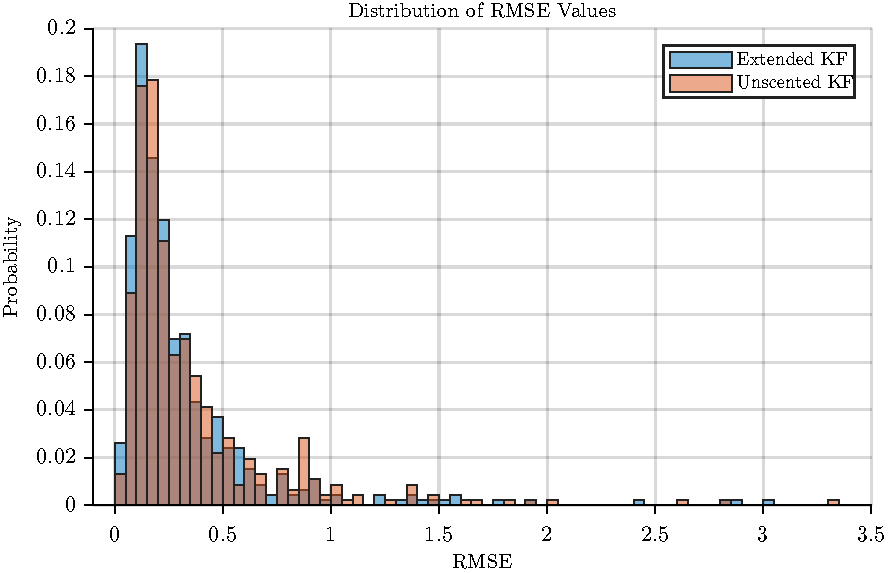
\includegraphics[width=\textwidth]{src/pics/EKFvsUKF_histogram.pdf}
	\caption{test}
	\label{fig:EKFvsUKF_histogram}
\end{figure}

The histogram shows that the performance of EKF and UKF is very similar.


% W20 plot
\begin{tikzpicture}
	\begin{groupplot}[
		ybar,
		group style={
			group size=2 by 1,
			horizontal sep=25pt,
			y descriptions at=edge left,
		},
		width=0.49\textwidth, height=6.5cm,
		symbolic x coords={0,5,10},
		xtick=data,
		xlabel={Wind Level $W_{20}$ [ft/s]},
		ymin=0, ymax=1.05,
		enlarge x limits=0.3,
		ymajorgrids, grid style={gray!25},
		tick align=outside,
		error bars/y dir=both,
		error bars/y explicit,
		error bars/error bar style={line width=0.8pt},
		legend style={draw=none, font=\small},
		legend pos=north west,
		]
		
		\nextgroupplot[title={All Estimates}, ylabel={RMSE}, bar width=10pt]
		\addplot+[fill=blue!55, draw=blue!70!black, error bars/.cd, y dir=both, y explicit]
		table[x=W20,y=mean,y error=std] {
			W20 mean std
			0 0.33912 0.28139
			5 0.39051 0.33253
			10 0.55392 0.42279
		};
		\addlegendentry{UKF}
		
		\addplot+[fill=orange!70, draw=orange!80!black, error bars/.cd, y dir=both, y explicit]
		table[x=W20,y=mean,y error=std] {
			W20 mean std
			0 0.26738 0.22207
			5 0.33867 0.30808
			10 0.53795 0.42298
		};
		\addlegendentry{EKF}
		
		\nextgroupplot[title={Converged Only}, bar width=10pt]
		\addplot+[fill=blue!55, draw=blue!70!black, error bars/.cd, y dir=both, y explicit]
		table[x=W20,y=mean,y error=std] {
			W20 mean std
			0 0.23895 0.28182
			5 0.31397 0.3292
			10 0.50904 0.44627
		};
		\addlegendentry{UKF}
		
		\addplot+[fill=orange!70, draw=orange!80!black, error bars/.cd, y dir=both, y explicit]
		table[x=W20,y=mean,y error=std] {
			W20 mean std
			0 0.18984 0.22752
			5 0.28108 0.32127
			10 0.50648 0.44631
		};
		\addlegendentry{EKF}
		
	\end{groupplot}
\end{tikzpicture}

the W20 barchart shows that obviously, more chellenging wind conditions, expressed by a higher wind reference value W20 result in a higher estimtion error.

\definecolor{ekfcolor}{RGB}{0,114,189}
\definecolor{ukfcolor}{RGB}{217,83,25}
% Boxplot
\begin{figure}[htbp]
	\centering
	\begin{tikzpicture}
		\begin{axis}[
			boxplot/draw direction=y,
			width=\textwidth, height=8.5cm,
			ylabel={Converged RMSE},
			xtick={0.3250,1.9750,3.6250,5.2750,6.9250,8.5750},
			xticklabels={curve,forward\_fast,forward\_slow,hover,rotate,sideways},
			x tick label style={rotate=0, align=center, font=\normalsize},
			xtick style={draw=none},
			xlabel={Scenario},
			xmin=-0.7500, xmax=9.6500,
			ymin=0, ymax=1.3,
			boxplot/whisker range=1.5,
			boxplot/box extend=0.50,
			xmajorgrids=false,
			ymajorgrids=true,
			grid style={gray!25},
			extra x ticks={1.1500,2.8000,4.4500,6.1000,7.7500},
			extra x tick labels={},
			extra x tick style={grid=major, major grid style={gray!35}, tick style={draw=none}},
			legend style={
				at={(0.98,0.98)}, anchor=north east,
				legend columns=1,
				fill=white, fill opacity=0.9, draw=black!40, text opacity=1,
			},
			]
			\addplot+[boxplot={draw position=0.0000}, mark=none, fill=ukfcolor!35, draw=ukfcolor, forget plot] table[row sep=\\, y index=0]{
				data\\
				1.6455\\
				0.66094\\
				0.52426\\
				0.45707\\
				0.48147\\
				3.3032\\
				0.67107\\
				0.39524\\
				0.24846\\
				0.205\\
				0.15512\\
				0.1688\\
				0.27806\\
				0.10735\\
				1.0137\\
				0.12265\\
				0.14883\\
				0.43337\\
				0.13614\\
				0.10403\\
				0.51807\\
				1.0433\\
				0.13236\\
				0.50571\\
				0.12875\\
				0.22046\\
				0.18439\\
				0.1331\\
				0.11075\\
				0.12953\\
				0.22689\\
				0.090022\\
				0.11588\\
				0.5578\\
				0.076722\\
				0.086142\\
				0.21262\\
				0.35377\\
				0.20138\\
				0.11622\\
				0.31811\\
				0.10374\\
				0.38458\\
				0.22071\\
				0.2005\\
				0.27758\\
				0.35358\\
				0.80038\\
				0.31837\\
				0.52403\\
				0.23034\\
				0.28814\\
				0.28815\\
				0.18842\\
				0.03682\\
				0.96804\\
				0.85102\\
				0.093897\\
				0.78722\\
				2.8216\\
				0.64682\\
				0.14068\\
				0.51763\\
				0.085096\\
			};
			\addplot+[boxplot={draw position=0.6500}, mark=none, fill=ekfcolor!35, draw=ekfcolor, forget plot] table[row sep=\\, y index=0]{
				data\\
				0.06501\\
				0.18696\\
				0.086482\\
				0.10426\\
				0.20459\\
				3.0481\\
				0.42963\\
				0.23607\\
				0.11483\\
				0.11292\\
				0.083522\\
				0.11002\\
				0.22596\\
				0.067406\\
				0.97564\\
				0.085966\\
				0.11255\\
				0.40115\\
				0.10432\\
				0.073013\\
				0.48901\\
				1.0168\\
				0.10664\\
				0.48012\\
				0.10357\\
				0.19586\\
				0.16085\\
				0.10988\\
				0.087835\\
				0.10778\\
				0.20551\\
				0.069443\\
				0.097508\\
				0.5419\\
				0.062427\\
				0.072002\\
				0.19952\\
				0.34237\\
				0.19062\\
				0.10563\\
				0.30761\\
				0.093602\\
				0.37453\\
				0.21077\\
				0.19258\\
				0.26976\\
				0.3471\\
				0.79484\\
				0.3129\\
				0.52087\\
				0.22742\\
				0.28599\\
				0.28737\\
				0.18916\\
				0.038149\\
				1.0078\\
				0.89465\\
				0.1382\\
				0.84137\\
				2.8835\\
				0.71884\\
				0.42101\\
				0.93194\\
				1.5862\\
			};
			\addplot+[boxplot={draw position=1.6500}, mark=none, fill=ukfcolor!35, draw=ukfcolor, forget plot] table[row sep=\\, y index=0]{
				data\\
				0.52391\\
				0.18938\\
				0.27621\\
				0.18521\\
				0.44113\\
				0.37721\\
				0.24301\\
				0.28604\\
				0.53588\\
				0.37072\\
				0.17449\\
				0.46987\\
				0.1367\\
				0.10392\\
				0.13645\\
				0.13463\\
				0.18321\\
				0.28549\\
				0.25061\\
				0.10046\\
				0.13589\\
				0.55732\\
				0.1802\\
				0.17506\\
				0.31351\\
				0.34443\\
				0.38165\\
				0.33072\\
				0.18071\\
				0.40461\\
				0.24266\\
				0.19613\\
				0.19914\\
				0.087049\\
				0.282\\
				0.091317\\
				0.40614\\
				0.021259\\
				0.38907\\
				0.1802\\
				0.59737\\
				0.27442\\
				0.24824\\
				0.090548\\
				0.090415\\
				0.19435\\
				0.19506\\
				0.20545\\
				0.13286\\
				0.33169\\
				0.18104\\
				0.34276\\
				0.28965\\
				0.11778\\
				0.33213\\
				0.1181\\
				0.1735\\
				0.013612\\
				0.22185\\
				0.12112\\
				0.20443\\
				0.13352\\
				0.34253\\
				0.12124\\
				0.079782\\
				0.30436\\
				0.46597\\
				0.27738\\
				0.078125\\
				0.1851\\
				0.13253\\
				1.3556\\
				1.9059\\
				0.20968\\
				1.2841\\
				0.17578\\
				0.15153\\
				0.15154\\
				0.06512\\
				0.12542\\
			};
			\addplot+[boxplot={draw position=2.3000}, mark=none, fill=ekfcolor!35, draw=ekfcolor, forget plot] table[row sep=\\, y index=0]{
				data\\
				0.48672\\
				0.15407\\
				0.24251\\
				0.15178\\
				0.40954\\
				0.34931\\
				0.21758\\
				0.26227\\
				0.51364\\
				0.34908\\
				0.15333\\
				0.45079\\
				0.11941\\
				0.086911\\
				0.12158\\
				0.11978\\
				0.1686\\
				0.27163\\
				0.23688\\
				0.086904\\
				0.12262\\
				0.54595\\
				0.16929\\
				0.16418\\
				0.30346\\
				0.3346\\
				0.37198\\
				0.32137\\
				0.17189\\
				0.39587\\
				0.23532\\
				0.18911\\
				0.19265\\
				0.080783\\
				0.27585\\
				0.08561\\
				0.40099\\
				0.016167\\
				0.38426\\
				0.17576\\
				0.59398\\
				0.27107\\
				0.24497\\
				0.087461\\
				0.087372\\
				0.19132\\
				0.1921\\
				0.20266\\
				0.1303\\
				0.32915\\
				0.17851\\
				0.34054\\
				0.28754\\
				0.11569\\
				0.33019\\
				0.11628\\
				0.17168\\
				0.011835\\
				0.22023\\
				0.12004\\
				0.20339\\
				0.13267\\
				0.34194\\
				0.12131\\
				0.080008\\
				0.30462\\
				0.4668\\
				0.27999\\
				0.081222\\
				0.19248\\
				0.14237\\
				1.3905\\
				1.9422\\
				0.26717\\
				1.343\\
				0.24277\\
				0.25547\\
				0.29857\\
				0.24247\\
				1.2423\\
			};
			\addplot+[boxplot={draw position=3.3000}, mark=none, fill=ukfcolor!35, draw=ukfcolor, forget plot] table[row sep=\\, y index=0]{
				data\\
				0.55459\\
				0.53396\\
				1.6947\\
				0.23052\\
				0.15504\\
				0.24631\\
				0.14507\\
				0.06372\\
				0.2431\\
				0.49322\\
				0.25523\\
				0.1235\\
				0.14229\\
				0.21396\\
				0.13974\\
				0.11747\\
				0.42923\\
				0.4741\\
				0.34392\\
				0.19644\\
				0.12527\\
				0.3841\\
				0.12214\\
				0.096633\\
				0.098187\\
				0.16583\\
				0.22213\\
				0.11738\\
				0.09363\\
				0.11694\\
				0.36707\\
				0.19816\\
				0.2148\\
				0.15946\\
				0.16114\\
				0.27879\\
				0.080197\\
				0.28702\\
				0.15289\\
				0.14728\\
				0.074609\\
				0.44315\\
				0.22463\\
				0.25336\\
				0.16045\\
				0.18048\\
				0.19614\\
				0.24505\\
				0.17744\\
				0.20164\\
				0.341\\
				0.090202\\
				0.18262\\
				0.090154\\
				0.12641\\
				0.35677\\
				0.10944\\
				0.16989\\
				0.36323\\
				0.019459\\
				0.10898\\
				0.11836\\
				0.25505\\
				0.3164\\
				0.10104\\
				0.1003\\
				0.15039\\
				0.32463\\
				0.069698\\
				0.050127\\
				0.32988\\
				0.19759\\
				0.22617\\
				0.3259\\
				1.3632\\
				1.4831\\
				0.44031\\
				0.069452\\
				1.3874\\
				0.29405\\
			};
			\addplot+[boxplot={draw position=3.9500}, mark=none, fill=ekfcolor!35, draw=ekfcolor, forget plot] table[row sep=\\, y index=0]{
				data\\
				0.075071\\
				0.38325\\
				1.5955\\
				0.17116\\
				0.10139\\
				0.19623\\
				0.10149\\
				0.021972\\
				0.2044\\
				0.45508\\
				0.21792\\
				0.089753\\
				0.11224\\
				0.18511\\
				0.1116\\
				0.08933\\
				0.40309\\
				0.44999\\
				0.32089\\
				0.17355\\
				0.10594\\
				0.36755\\
				0.10603\\
				0.082255\\
				0.083855\\
				0.15163\\
				0.20801\\
				0.10494\\
				0.082216\\
				0.10557\\
				0.3558\\
				0.18699\\
				0.20378\\
				0.14921\\
				0.15098\\
				0.26916\\
				0.070642\\
				0.27789\\
				0.14431\\
				0.13899\\
				0.066385\\
				0.43493\\
				0.21728\\
				0.24639\\
				0.15367\\
				0.17406\\
				0.19091\\
				0.24116\\
				0.17362\\
				0.19845\\
				0.33834\\
				0.087578\\
				0.18002\\
				0.087706\\
				0.12409\\
				0.35468\\
				0.10761\\
				0.16807\\
				0.3615\\
				0.017952\\
				0.10747\\
				0.11731\\
				0.25416\\
				0.31568\\
				0.10063\\
				0.099935\\
				0.15038\\
				0.32462\\
				0.071134\\
				0.052981\\
				0.33455\\
				0.20387\\
				0.23487\\
				0.33613\\
				1.3785\\
				1.5002\\
				0.45844\\
				0.087806\\
				1.4169\\
				0.32748\\
			};
			\addplot+[boxplot={draw position=4.9500}, mark=none, fill=ukfcolor!35, draw=ukfcolor, forget plot] table[row sep=\\, y index=0]{
				data\\
				2.0284\\
				0.91074\\
				0.91819\\
				0.85833\\
				1.1098\\
				0.85836\\
				1.0015\\
				0.928\\
				0.92225\\
				0.6953\\
				0.89885\\
				0.78329\\
				0.76758\\
				0.87819\\
				0.86908\\
				0.86766\\
				1.0359\\
				0.806\\
				0.86212\\
				0.98388\\
				0.42471\\
				0.42264\\
				0.76441\\
				0.79664\\
				1.0656\\
				0.75424\\
				0.43732\\
				0.43497\\
				0.3745\\
				0.50145\\
				0.93838\\
				0.65194\\
				1.1052\\
				0.37154\\
				0.39215\\
				0.8294\\
				0.86687\\
				0.38107\\
				0.32033\\
				0.86995\\
				0.35641\\
				0.20015\\
				0.34799\\
				0.64816\\
				0.77037\\
				0.21681\\
				0.60868\\
				0.89245\\
				0.64029\\
				0.60123\\
				0.48006\\
				0.19991\\
				0.42334\\
				0.62248\\
				0.43247\\
				0.43091\\
				0.11506\\
				0.66795\\
				0.52017\\
				0.41721\\
				0.51368\\
				0.20488\\
				0.070793\\
				0.33955\\
				0.37375\\
				0.056544\\
				0.67806\\
				0.18833\\
				0.36577\\
				0.15807\\
				0.50282\\
				0.31599\\
				0.41649\\
				0.49014\\
				0.47368\\
				0.85058\\
				0.51626\\
				0.36887\\
				0.31771\\
				0.3334\\
				0.21952\\
			};
			\addplot+[boxplot={draw position=5.6000}, mark=none, fill=ekfcolor!35, draw=ekfcolor, forget plot] table[row sep=\\, y index=0]{
				data\\
				0.91978\\
				0.48149\\
				0.49538\\
				0.50644\\
				0.76546\\
				0.51489\\
				0.65872\\
				0.59101\\
				0.58925\\
				0.3851\\
				0.60427\\
				0.49163\\
				0.47808\\
				0.60268\\
				0.60364\\
				0.60321\\
				0.77605\\
				0.57429\\
				0.63364\\
				0.75793\\
				0.21307\\
				0.21881\\
				0.5667\\
				0.60348\\
				0.87412\\
				0.56466\\
				0.25504\\
				0.2591\\
				0.20619\\
				0.33563\\
				0.77319\\
				0.49075\\
				0.94534\\
				0.21173\\
				0.25659\\
				0.69525\\
				0.74178\\
				0.25993\\
				0.2048\\
				0.75883\\
				0.24889\\
				0.098034\\
				0.24718\\
				0.55955\\
				0.68435\\
				0.13128\\
				0.52471\\
				0.80855\\
				0.5634\\
				0.53063\\
				0.40951\\
				0.13343\\
				0.36069\\
				0.56246\\
				0.37294\\
				0.3849\\
				0.080136\\
				0.63718\\
				0.49084\\
				0.38868\\
				0.48533\\
				0.17932\\
				0.049421\\
				0.31891\\
				0.36545\\
				0.049246\\
				0.67728\\
				0.2042\\
				0.38698\\
				0.18107\\
				0.52658\\
				0.34221\\
				0.44976\\
				0.53205\\
				0.52931\\
				0.92233\\
				0.59335\\
				0.45704\\
				0.41108\\
				0.45657\\
				0.38826\\
			};
			\addplot+[boxplot={draw position=6.6000}, mark=none, fill=ukfcolor!35, draw=ukfcolor, forget plot] table[row sep=\\, y index=0]{
				data\\
				1.8433\\
				0.20372\\
				0.18229\\
				0.23742\\
				0.093248\\
				0.08723\\
				0.15738\\
				0.31385\\
				0.094929\\
				0.28711\\
				0.2748\\
				0.12787\\
				0.064407\\
				0.30704\\
				0.13001\\
				0.095743\\
				0.1561\\
				0.1355\\
				0.082693\\
				0.16502\\
				0.12334\\
				0.075\\
				0.1331\\
				0.19346\\
				0.17929\\
				0.1627\\
				0.13341\\
				0.12924\\
				0.28373\\
				0.14986\\
				0.1724\\
				0.21438\\
				0.12972\\
				0.32251\\
				0.14193\\
				0.18754\\
				0.10682\\
				0.17686\\
				0.19829\\
				0.25139\\
				0.095476\\
				0.1694\\
				0.13781\\
				0.13957\\
				0.24811\\
				0.17048\\
				0.22691\\
				0.2488\\
				0.22583\\
				0.16045\\
				0.26371\\
				0.2467\\
				0.17301\\
				0.14834\\
				0.14153\\
				0.2706\\
				0.28424\\
				0.18739\\
				0.267\\
				0.1658\\
				0.40432\\
				0.11961\\
				0.19783\\
				0.3765\\
				0.13523\\
				0.89931\\
				0.093453\\
				0.24319\\
				0.33531\\
				0.19723\\
				0.16599\\
				0.16062\\
				0.14479\\
				0.64543\\
				0.63567\\
				1.3981\\
			};
			\addplot+[boxplot={draw position=7.2500}, mark=none, fill=ekfcolor!35, draw=ekfcolor, forget plot] table[row sep=\\, y index=0]{
				data\\
				1.7554\\
				0.11868\\
				0.10643\\
				0.17667\\
				0.033473\\
				0.031055\\
				0.11847\\
				0.27784\\
				0.05921\\
				0.25277\\
				0.24358\\
				0.10277\\
				0.041945\\
				0.28466\\
				0.1085\\
				0.075768\\
				0.13703\\
				0.11663\\
				0.064901\\
				0.14789\\
				0.10782\\
				0.059653\\
				0.11779\\
				0.17873\\
				0.16482\\
				0.14825\\
				0.11974\\
				0.11613\\
				0.27262\\
				0.13902\\
				0.16202\\
				0.20438\\
				0.11989\\
				0.31285\\
				0.13248\\
				0.17825\\
				0.097524\\
				0.16785\\
				0.18959\\
				0.24371\\
				0.088022\\
				0.16212\\
				0.13056\\
				0.13238\\
				0.24093\\
				0.16349\\
				0.22103\\
				0.24365\\
				0.22139\\
				0.15614\\
				0.25987\\
				0.24287\\
				0.16922\\
				0.14473\\
				0.13805\\
				0.26717\\
				0.28159\\
				0.18511\\
				0.26514\\
				0.16461\\
				0.40362\\
				0.12001\\
				0.19856\\
				0.37727\\
				0.13692\\
				0.90315\\
				0.10064\\
				0.25372\\
				0.34964\\
				0.21681\\
				0.22481\\
				0.22698\\
				0.21918\\
				0.86941\\
				1.2214\\
				2.4402\\
			};
			\addplot+[boxplot={draw position=8.2500}, mark=none, fill=ukfcolor!35, draw=ukfcolor, forget plot] table[row sep=\\, y index=0]{
				data\\
				0.22543\\
				0.39746\\
				0.38989\\
				0.32044\\
				0.3686\\
				0.15715\\
				0.17002\\
				0.14611\\
				0.1696\\
				0.16887\\
				0.17016\\
				0.1639\\
				0.16188\\
				0.21085\\
				0.14745\\
				0.61958\\
				0.18309\\
				0.12962\\
				0.15944\\
				0.24577\\
				0.19994\\
				0.11555\\
				0.34235\\
				0.10815\\
				0.078593\\
				0.11777\\
				0.16722\\
				0.2289\\
				0.12761\\
				0.13369\\
				0.13723\\
				0.074319\\
				0.21658\\
				0.21804\\
				0.13534\\
				0.40986\\
				0.06748\\
				0.12998\\
				0.13453\\
				0.099665\\
				0.16573\\
				0.1956\\
				0.30655\\
				0.196\\
				0.24606\\
				0.33677\\
				0.17403\\
				0.23171\\
				0.17718\\
				0.25109\\
				0.12412\\
				0.15294\\
				0.2709\\
				0.11729\\
				0.24312\\
				0.10445\\
				0.13084\\
				0.23164\\
				0.2002\\
				1.4584\\
				0.028549\\
				0.17489\\
				0.18029\\
				0.094525\\
				0.06056\\
				0.025707\\
				0.17408\\
				0.18226\\
				0.13349\\
				0.44646\\
				0.29074\\
				0.3718\\
				0.13858\\
				0.21448\\
				0.34359\\
				0.33974\\
				0.05311\\
				0.47263\\
				2.6489\\
			};
			\addplot+[boxplot={draw position=8.9000}, mark=none, fill=ekfcolor!35, draw=ekfcolor, forget plot] table[row sep=\\, y index=0]{
				data\\
				0.13432\\
				0.31294\\
				0.33221\\
				0.27071\\
				0.32821\\
				0.12013\\
				0.1339\\
				0.11271\\
				0.13964\\
				0.13901\\
				0.14316\\
				0.13709\\
				0.13665\\
				0.18655\\
				0.12431\\
				0.59682\\
				0.16048\\
				0.10761\\
				0.13954\\
				0.22601\\
				0.18114\\
				0.097164\\
				0.3254\\
				0.091877\\
				0.062475\\
				0.10373\\
				0.15401\\
				0.21606\\
				0.11484\\
				0.12165\\
				0.12556\\
				0.062889\\
				0.20526\\
				0.20706\\
				0.12457\\
				0.39909\\
				0.056912\\
				0.1197\\
				0.12596\\
				0.091719\\
				0.15846\\
				0.18836\\
				0.29951\\
				0.18937\\
				0.2395\\
				0.33031\\
				0.16769\\
				0.22561\\
				0.17132\\
				0.24544\\
				0.11872\\
				0.14762\\
				0.26571\\
				0.11266\\
				0.23855\\
				0.099962\\
				0.1265\\
				0.22776\\
				0.19723\\
				1.4561\\
				0.026643\\
				0.17312\\
				0.17857\\
				0.092965\\
				0.059951\\
				0.025162\\
				0.17403\\
				0.18296\\
				0.13425\\
				0.44803\\
				0.29343\\
				0.37451\\
				0.14136\\
				0.21794\\
				0.3472\\
				0.34391\\
				0.059552\\
				0.48356\\
				2.81\\
			};
			\addlegendimage{area legend, fill=ekfcolor!35, draw=ekfcolor}
			\addlegendentry{Extended KF}
			\addlegendimage{area legend, fill=ukfcolor!35, draw=ukfcolor}
			\addlegendentry{Unscented KF}
		\end{axis}
	\end{tikzpicture}
	\caption{Mean RMSE by scenario for Unscented KF and Extended KF. Boxes show the interquartile range (Q1--Q3) with the median line; whiskers extend to the most extreme point within 1.5$\times$IQR. Outlier points beyond the whiskers are omitted.}
	\label{fig:rmse-converged}
\end{figure}

The boxplot specifically show that hovering is the most challenging mode to be in, this can be because the velocity is equal to zero for this mode and theres no velocity information, which gives the wind estimation a good freedom.
Find out: For hover: is the value bad for all W20 or only for constant wind?

In combination with the W20 plot that shows that the problem is not constant wind but the combination of (const wind through V = 0) and no velocity V = 0. More precisely no new wind information is delievered (compared to rotation for ex.) so a equilibrium can set with wrong wind comp.
And only NDI has this problem as there we directly consider Va, whereas the DFF explicitly computes Faero with and without wind


\subsection{Effect of Airspeed Sensor}
The Airship is equipped with an 1-D airspeed sensor. Its interesting to know how the wind estimation changes if no airspeed sensor is in place, to quantify the importance of the AS.

\todo{include one time plot and one numeric comparision}





\section{Wind compensation}
\label{sec:5.2WindCompensation}

Compensation method has influence on the wind estimation as well. 

\begin{figure}[htbp]
	\centering
	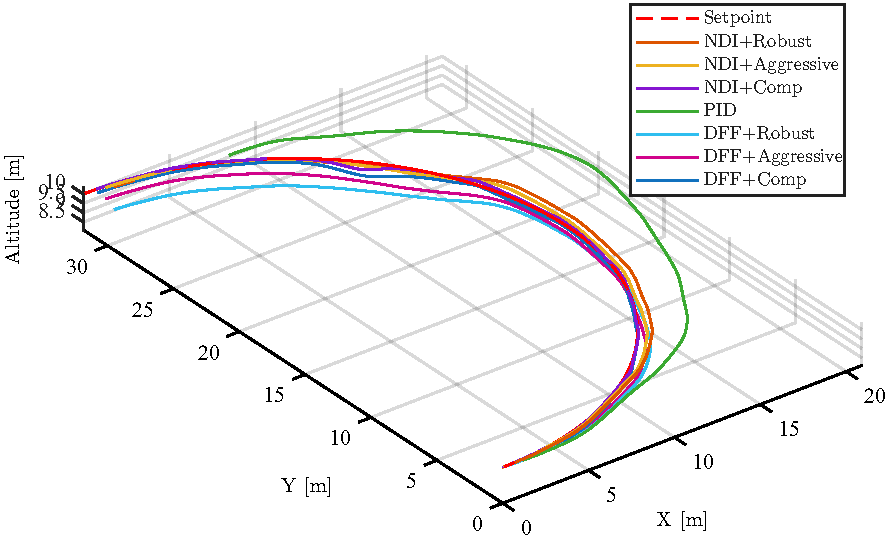
\includegraphics[width=\textwidth]{src/pics/Compensation_Trajectory_5_25_0_0.pdf}
	\caption{Comparision of wind estimation performance for different estimated W20, W20 actual is 5.}
	\label{fig:my_figure}
\end{figure}

\begin{figure}[htbp]
	\centering
	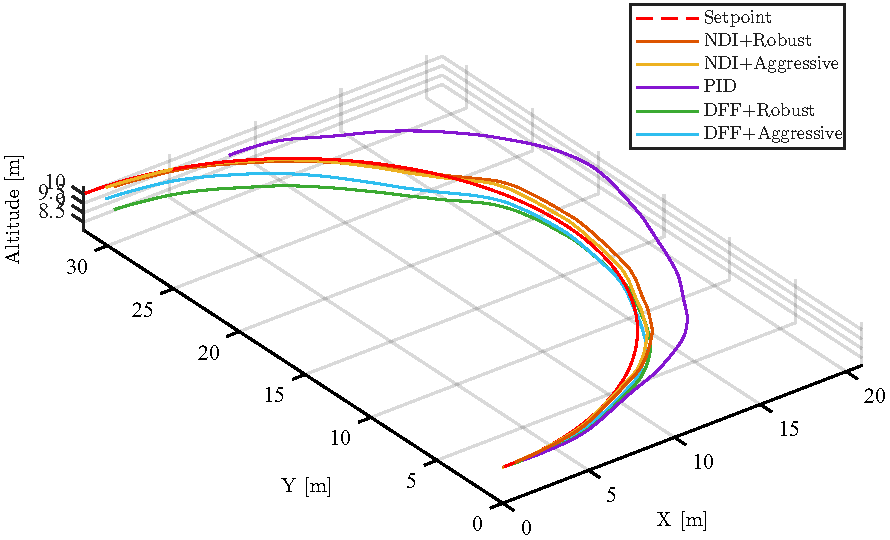
\includegraphics[width=\textwidth]{src/pics/Compensation_Trajectory_5_25_0_0_noCompGains.pdf}
	\caption{Comparision of wind estimation performance for different estimated W20, W20 actual is 5.}
	\label{fig:my_figure}
\end{figure}

To enable a fair comparison of the evaluated controller and gain combinations across flight scenarios, the raw RMSE values are first normalized and subsequently aggregated into a single scale-independent performance metric. This step is necessary because the twelve tracked state variables --- position, velocity, attitude, and angular rate errors --- differ substantially in both physical units and magnitude (e.g.\ position errors on the order of meters versus attitude errors on the order of radians), such that a direct average of the raw RMSE values would be dominated by the variables with the largest absolute scale.

\paragraph{Normalization.}
For a given scenario $s$, the mean RMSE of variable $v$ is computed across all $M$ evaluated controller/gain combinations:
\begin{equation}
	\overline{\mathrm{RMSE}}_{s,v} = \frac{1}{M}\sum_{m=1}^{M} \mathrm{RMSE}_{s,m,v}
	\label{eq:scenario_mean}
\end{equation}
Each raw RMSE value is then expressed relative to this scenario- and variable-specific reference:
\begin{equation}
	\widetilde{\mathrm{RMSE}}_{s,m,v} = \frac{\mathrm{RMSE}_{s,m,v}}{\overline{\mathrm{RMSE}}_{s,v}}
	\label{eq:norm_rmse}
\end{equation}
A normalized value of $\widetilde{\mathrm{RMSE}}_{s,m,v} = 1$ therefore corresponds to average performance for that scenario and variable, while values below and above $1$ indicate above- and below-average estimation or control accuracy, respectively.

\paragraph{Aggregation.}
Since the normalized quantities in Eq.~\eqref{eq:norm_rmse} are dimensionless and share a common reference (the scenario average), they can be meaningfully averaged across all $V = 12$ state variables to obtain a single figure of merit per scenario and controller/gain combination:
\begin{equation}
	\overline{\widetilde{\mathrm{RMSE}}}_{s,m} = \frac{1}{V}\sum_{v=1}^{V} \widetilde{\mathrm{RMSE}}_{s,m,v}
	\label{eq:avg_norm_rmse}
\end{equation}
This average normalized RMSE weights each state variable equally regardless of its native units or magnitude, and is used throughout Section~\ref{sec:results} to compare the relative performance of the PID, NDI, and DFF control architectures under the Aggressive, Comp, and Robust gain settings.


% original	
%\begin{figure}[htbp]
%	
%	\centering
%	
%	\definecolor{barblue}{RGB}{55,138,221}
%	\definecolor{barmatch}{RGB}{216,90,48}
%	
%	\pgfplotsset{
%		rmse bar/.style={
%			ybar,
%			bar width=14pt,
%			width=\linewidth,
%			height=5cm,
%			enlarge x limits=0.12,
%			xlabel={Method--Gains combination},
%			ylabel={Avg.\ norm.\ RMSE},
%			ymin=0,
%			ymax=2.1,
%			xticklabel style={font=\small},
%			yticklabel style={font=\small},
%			xlabel style={font=\small},
%			ylabel style={font=\small},
%			ymajorgrids=true,
%			bar shift=0pt,
%			grid style={gray!20}
%		}
%	}
%	
%	% ----- curve -----
%	\begin{subfigure}[b]{0.48\textwidth}
%		\centering
%		\begin{tikzpicture}
%			\begin{axis}[rmse bar, title={curve},
%				symbolic x coords={N-C,C-C,C-R,PID,C-A,N-R,N-A}, xtick=data,
%				xticklabels={N-C,C-C,C-R,PID,C-A,N-R,N-A}]
%				\addplot[fill=barblue] coordinates {
%					(N-C,1.3046)(C-C,1.1951)(C-R,0.9692)(PID,0.9668)(C-A,0.9541)(N-R,0.8465)(N-A,0.7636)
%				};
%				\addplot[fill=barmatch] coordinates { (N-R,0.8465) };
%			\end{axis}
%		\end{tikzpicture}
%	\end{subfigure}
%	\hfill
%	% ----- forward_fast -----
%	\begin{subfigure}[t]{0.48\textwidth}
%		\centering
%		\begin{tikzpicture}
%			\begin{axis}[rmse bar, title={forward\_fast},
%				symbolic x coords={N-C,C-C,C-R,C-A,PID,N-R,N-A}, xtick=data,
%				xticklabels={N-C,C-C,C-R,C-A,PID,N-R,N-A}]
%				\addplot[fill=barblue] coordinates {
%					(N-C,1.2795)(C-C,1.2168)(C-R,0.9572)(C-A,0.9168)(PID,0.9009)(N-R,0.8696)(N-A,0.8593)
%				};
%				\addplot[fill=barmatch] coordinates { (N-R,0.8696) };
%			\end{axis}
%		\end{tikzpicture}
%	\end{subfigure}
%	
%	\vspace{1em}
%	
%	% ----- forward_slow -----
%	\begin{subfigure}[t]{0.48\textwidth}
%		\centering
%		\begin{tikzpicture}
%			\begin{axis}[rmse bar, title={forward\_slow},
%				symbolic x coords={N-C,C-C,C-A,N-A,C-R,PID,N-R}, xtick=data,
%				xticklabels={N-C,C-C,C-A,N-A,C-R,PID,N-R}]
%				\addplot[fill=barblue] coordinates {
%					(N-C,1.2116)(C-C,1.1496)(C-A,1.1001)(N-A,1.0368)(C-R,0.9436)(PID,0.9023)(N-R,0.6558)
%				};
%				\addplot[fill=barmatch] coordinates { (N-R,0.6558) };
%			\end{axis}
%		\end{tikzpicture}
%	\end{subfigure}
%	\hfill
%	% ----- hover -----
%	\begin{subfigure}[t]{0.48\textwidth}
%		\centering
%		\begin{tikzpicture}
%			\begin{axis}[rmse bar, title={hover},
%				symbolic x coords={C-R,N-R,PID,N-A,N-C,C-A,C-C}, xtick=data,
%				xticklabels={C-R,N-R,PID,N-A,N-C,C-A,C-C}]
%				\addplot[fill=barblue] coordinates {
%					(C-R,1.3350)(N-R,1.3185)(PID,1.1810)(N-A,1.0249)(N-C,0.8214)(C-A,0.7574)(C-C,0.5617)
%				};
%				\addplot[fill=barmatch] coordinates { (N-R,1.3185) };
%			\end{axis}
%		\end{tikzpicture}
%	\end{subfigure}
%	
%	\vspace{1em}
%	
%	% ----- rotate -----
%	\begin{subfigure}[t]{0.48\textwidth}
%		\centering
%		\begin{tikzpicture}
%			\begin{axis}[rmse bar, title={rotate},
%				symbolic x coords={PID,N-A,C-R,C-C,N-R,C-A,N-C}, xtick=data,
%				xticklabels={PID,N-A,C-R,C-C,N-R,C-A,N-C}]
%				\addplot[fill=barblue] coordinates {
%					(PID,1.9527)(N-A,1.6681)(C-R,1.1019)(C-C,0.6308)(N-R,0.6116)(C-A,0.5517)(N-C,0.4831)
%				};
%				\addplot[fill=barmatch] coordinates { (N-R,0.6116) };
%			\end{axis}
%		\end{tikzpicture}
%	\end{subfigure}
%	\hfill
%	% ----- sideways -----
%	\begin{subfigure}[t]{0.48\textwidth}
%		\centering
%		\begin{tikzpicture}
%			\begin{axis}[rmse bar, title={sideways},
%				symbolic x coords={N-C,C-C,C-A,C-R,N-A,N-R,PID}, xtick=data,
%				xticklabels={N-C,C-C,C-A,C-R,N-A,N-R,PID}]
%				\addplot[fill=barblue] coordinates {
%					(N-C,1.5194)(C-C,1.4888)(C-A,1.1268)(C-R,0.8853)(N-A,0.8138)(N-R,0.6836)(PID,0.4823)
%				};
%				\addplot[fill=barmatch] coordinates { (N-R,0.6836) };
%			\end{axis}
%		\end{tikzpicture}
%	\end{subfigure}
%	
%	\caption{Comparison of average normalized RMSE across all controller/gain combinations for each flight scenario, sorted from highest to lowest. The orange bar highlights the NDI controller with Robust gains.}
%	\label{fig:rmse_barchart}
%\end{figure}

% gekürzt
\begin{figure}[htbp]
	
	\centering
	
	\definecolor{barblue}{RGB}{55,138,221}
	\definecolor{barmatch}{RGB}{216,90,48}
	
	\pgfplotsset{
		rmse bar/.style={
			ybar,
			bar width=18pt,
			width=\linewidth,
			height=5cm,
			enlarge x limits=0.12,
			xlabel={Method--Gains combination},
			ylabel={Avg.\ norm.\ RMSE},
			ymin=0,
			ymax=2.1,
			xticklabel style={font=\small},
			yticklabel style={font=\small},
			xlabel style={font=\small},
			ylabel style={font=\small},
			ymajorgrids=true,
			bar shift=0pt,
			grid style={gray!20}
		}
	}
	
	% ----- curve -----
	\begin{subfigure}[b]{0.48\textwidth}
		\centering
		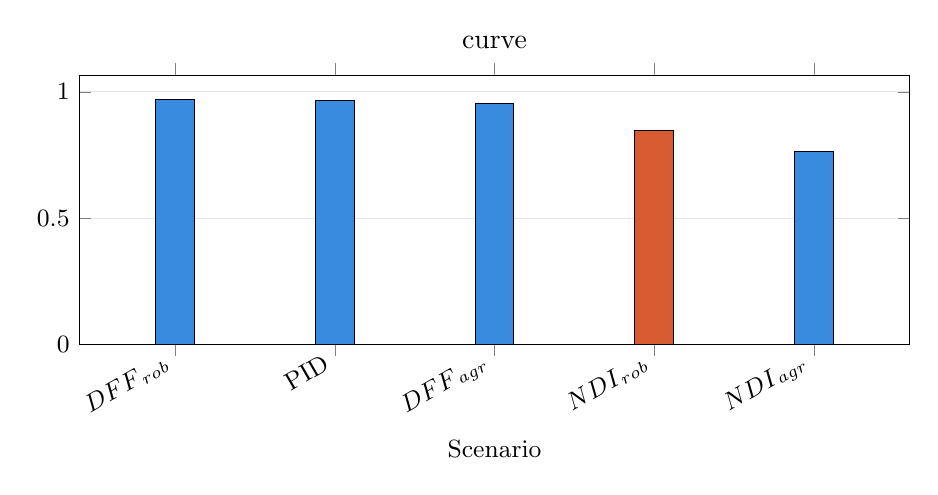
\begin{tikzpicture}
			\begin{axis}[rmse bar, title={curve},
				symbolic x coords={C-R,PID,C-A,N-R,N-A}, xtick=data,
				xticklabels={$\text{DFF}_\text{rob}$,PID,$\text{DFF}_\text{agr}$,$\text{NDI}_\text{rob}$,$\text{NDI}_\text{agr}$}]
				\addplot[fill=barblue] coordinates {
					(C-R,0.9692)(PID,0.9668)(C-A,0.9541)(N-R,0.8465)(N-A,0.7636)
				};
				\addplot[fill=barmatch] coordinates { (N-R,0.8465) };
			\end{axis}
		\end{tikzpicture}
	\end{subfigure}
	\hfill
	% ----- forward_fast -----
	\begin{subfigure}[t]{0.48\textwidth}
		\centering
		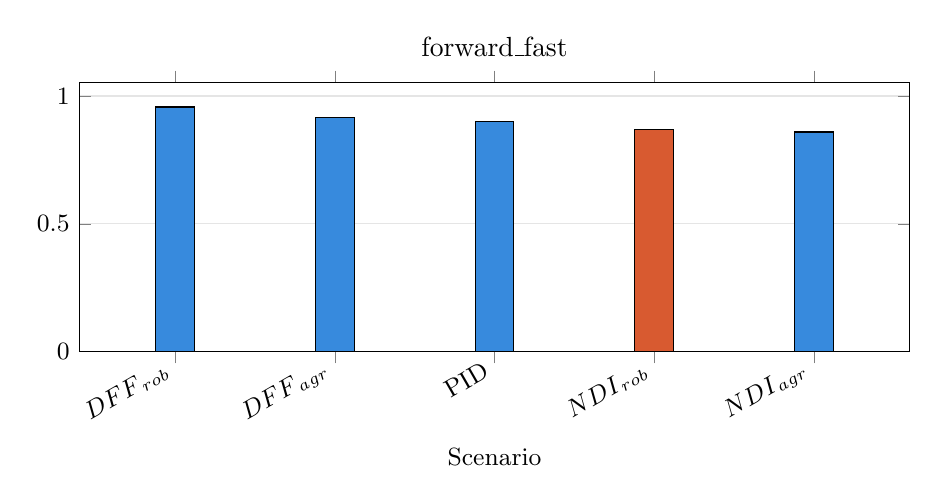
\begin{tikzpicture}
			\begin{axis}[rmse bar, title={forward\_fast},
				symbolic x coords={C-R,C-A,PID,N-R,N-A}, xtick=data,
				xticklabels={$\text{DFF}_\text{rob}$,$\text{DFF}_\text{agr}$,PID,$\text{NDI}_\text{rob}$,$\text{NDI}_\text{agr}$}]
				\addplot[fill=barblue] coordinates {
					(C-R,0.9572)(C-A,0.9168)(PID,0.9009)(N-R,0.8696)(N-A,0.8593)
				};
				\addplot[fill=barmatch] coordinates { (N-R,0.8696) };
			\end{axis}
		\end{tikzpicture}
	\end{subfigure}
	
	\vspace{1em}
	
	% ----- forward_slow -----
	\begin{subfigure}[t]{0.48\textwidth}
		\centering
		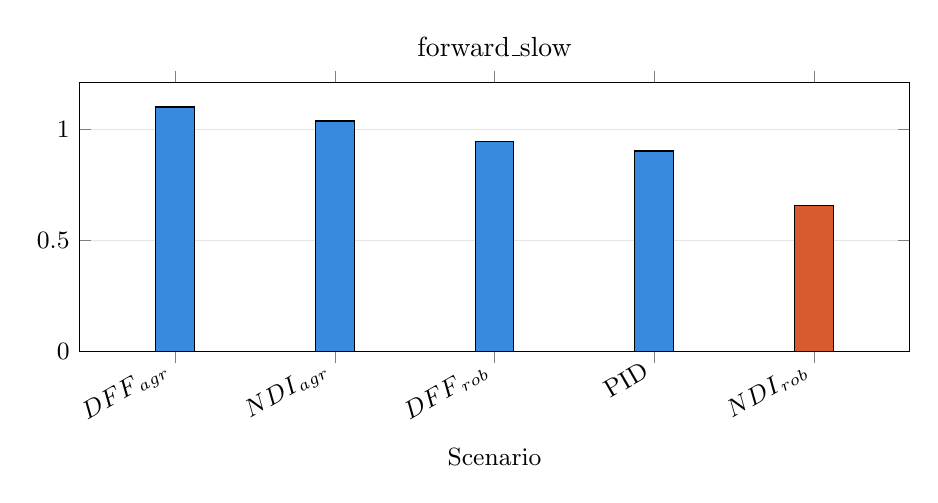
\begin{tikzpicture}
			\begin{axis}[rmse bar, title={forward\_slow},
				symbolic x coords={C-A,N-A,C-R,PID,N-R}, xtick=data,
				xticklabels={$\text{DFF}_\text{agr}$,$\text{NDI}_\text{agr}$,$\text{DFF}_\text{rob}$,PID,$\text{NDI}_\text{rob}$}]
				\addplot[fill=barblue] coordinates {
					(C-A,1.1001)(N-A,1.0368)(C-R,0.9436)(PID,0.9023)(N-R,0.6558)
				};
				\addplot[fill=barmatch] coordinates { (N-R,0.6558) };
			\end{axis}
		\end{tikzpicture}
	\end{subfigure}
	\hfill
	% ----- hover -----
	\begin{subfigure}[t]{0.48\textwidth}
		\centering
		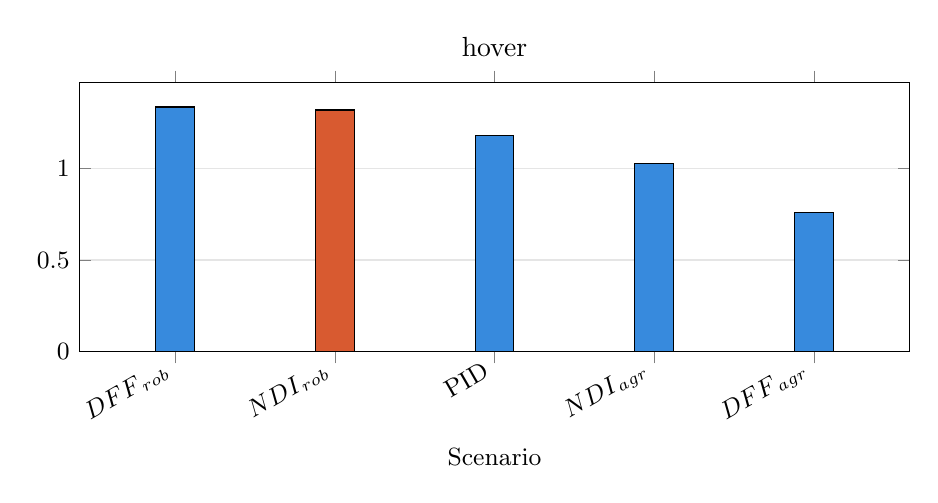
\begin{tikzpicture}
			\begin{axis}[rmse bar, title={hover},
				symbolic x coords={C-R,N-R,PID,N-A,C-A}, xtick=data,
				xticklabels={$\text{DFF}_\text{rob}$,$\text{NDI}_\text{rob}$,PID,$\text{NDI}_\text{agr}$,$\text{DFF}_\text{agr}$}]
				\addplot[fill=barblue] coordinates {
					(C-R,1.3350)(N-R,1.3185)(PID,1.1810)(N-A,1.0249)(C-A,0.7574)
				};
				\addplot[fill=barmatch] coordinates { (N-R,1.3185) };
			\end{axis}
		\end{tikzpicture}
	\end{subfigure}
	
	\vspace{1em}
	
	% ----- rotate -----
	\begin{subfigure}[t]{0.48\textwidth}
		\centering
		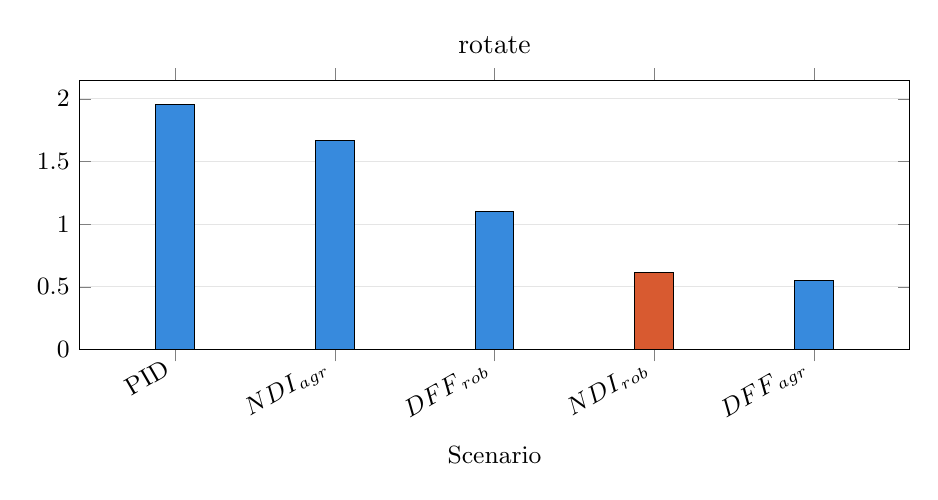
\begin{tikzpicture}
			\begin{axis}[rmse bar, title={rotate},
				symbolic x coords={PID,N-A,C-R,N-R,C-A}, xtick=data,
				xticklabels={PID,$\text{NDI}_\text{agr}$,$\text{DFF}_\text{rob}$,$\text{NDI}_\text{rob}$,$\text{DFF}_\text{agr}$}]
				\addplot[fill=barblue] coordinates {
					(PID,1.9527)(N-A,1.6681)(C-R,1.1019)(N-R,0.6116)(C-A,0.5517)
				};
				\addplot[fill=barmatch] coordinates { (N-R,0.6116) };
			\end{axis}
		\end{tikzpicture}
	\end{subfigure}
	\hfill
	% ----- sideways -----
	\begin{subfigure}[t]{0.48\textwidth}
		\centering
		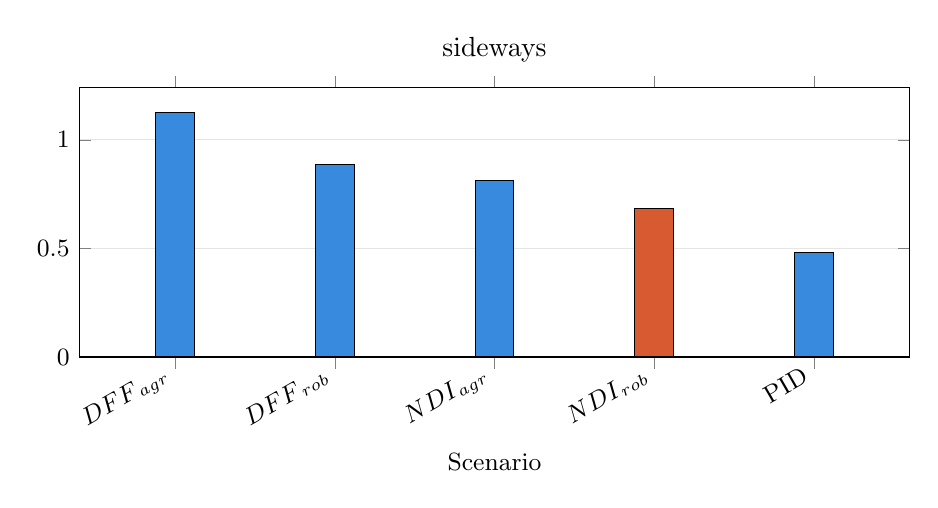
\begin{tikzpicture}
			\begin{axis}[rmse bar, title={sideways},
				symbolic x coords={C-A,C-R,N-A,N-R,PID}, xtick=data,
				xticklabels={$\text{DFF}_\text{agr}$,$\text{DFF}_\text{rob}$,$\text{NDI}_\text{agr}$,$\text{NDI}_\text{rob}$,PID}]
				\addplot[fill=barblue] coordinates {
					(C-A,1.1268)(C-R,0.8853)(N-A,0.8138)(N-R,0.6836)(PID,0.4823)
				};
				\addplot[fill=barmatch] coordinates { (N-R,0.6836) };
			\end{axis}
		\end{tikzpicture}
	\end{subfigure}
	
	\caption{Comparison of average normalized RMSE across selected controller/gain combinations for each flight scenario, sorted from highest to lowest. The orange bar highlights the NDI controller with Robust gains. The combinations NDI-Comp and DFF-Comp have been left out for better clarity.}
	\label{fig:rmse_barchart}
\end{figure}


\begin{figure}[htbp]
	
	\centering
	
	\definecolor{barblue}{RGB}{55,138,221}
	
	\pgfplotsset{
		rmse bar/.style={
			ybar,
			bar width=14pt,
			width=\linewidth,
			height=5cm,
			enlarge x limits=0.15,
			xlabel={Scenario},
			ymin=0,
			xticklabel style={font=\small, rotate=30, anchor=east},
			yticklabel style={font=\small},
			xlabel style={font=\small},
			ylabel style={font=\small},
			ymajorgrids=true,
			bar shift=0pt,
			grid style={gray!20},
			symbolic x coords={curve,forward\_fast,forward\_slow,hover,rotate,sideways},
			xtick=data,
		}
	}
	
	% ----- RMSE Pos -----
	\begin{subfigure}[b]{0.48\textwidth}
		\centering
		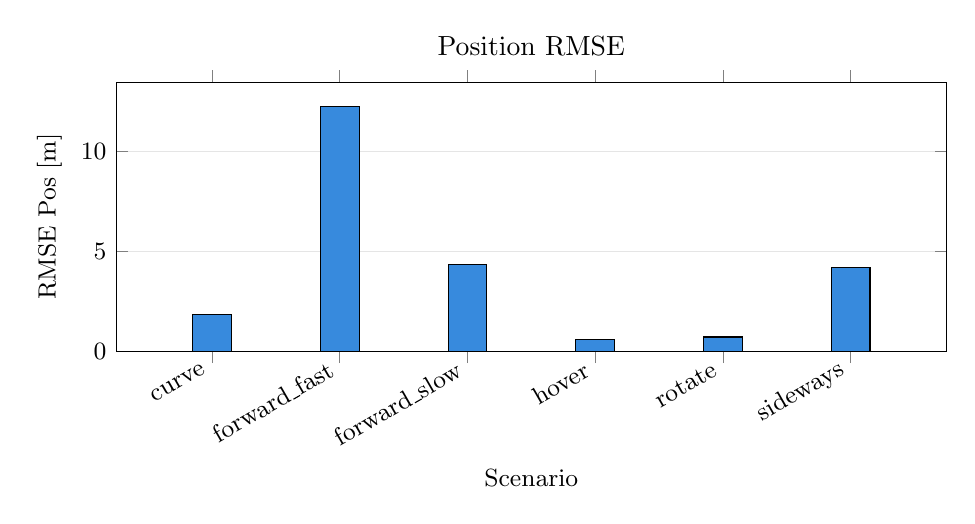
\begin{tikzpicture}
			\begin{axis}[rmse bar, title={Position RMSE}, ylabel={RMSE Pos [m]}]
				\addplot[fill=barblue] coordinates {
					(curve,1.8576)(forward\_fast,12.2179)(forward\_slow,4.3261)
					(hover,0.5762)(rotate,0.7193)(sideways,4.1662)
				};
			\end{axis}
		\end{tikzpicture}
	\end{subfigure}
	\hfill
	% ----- RMSE Vel -----
	\begin{subfigure}[b]{0.48\textwidth}
		\centering
		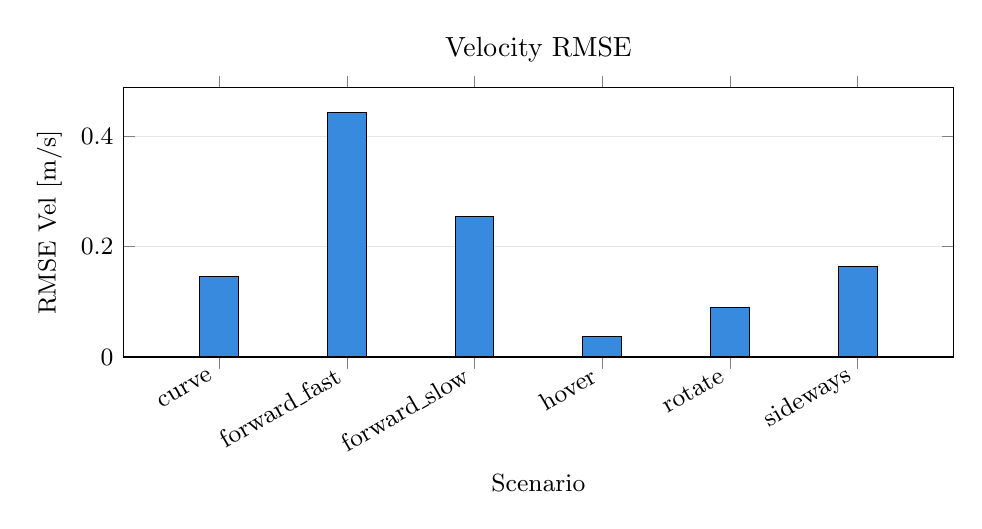
\begin{tikzpicture}
			\begin{axis}[rmse bar, title={Velocity RMSE}, ylabel={RMSE Vel [m/s]}]
				\addplot[fill=barblue] coordinates {
					(curve,0.1455)(forward\_fast,0.4434)(forward\_slow,0.2550)
					(hover,0.0367)(rotate,0.0890)(sideways,0.1634)
				};
			\end{axis}
		\end{tikzpicture}
	\end{subfigure}
	
	\vspace{1em}
	
	% ----- RMSE Att -----
	\begin{subfigure}[b]{0.48\textwidth}
		\centering
		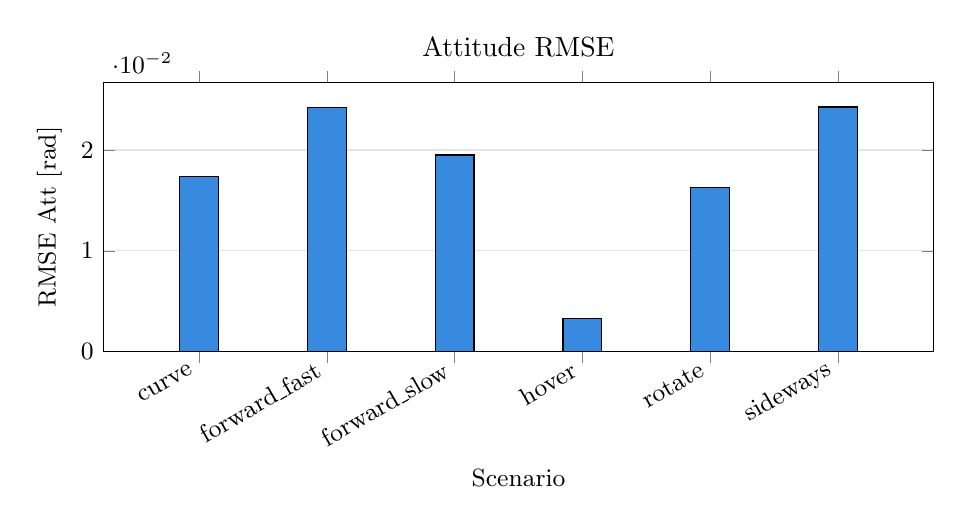
\begin{tikzpicture}
			\begin{axis}[rmse bar, title={Attitude RMSE}, ylabel={RMSE Att [rad]}]
				\addplot[fill=barblue] coordinates {
					(curve,0.01733)(forward\_fast,0.02420)(forward\_slow,0.01951)
					(hover,0.00325)(rotate,0.01631)(sideways,0.02427)
				};
			\end{axis}
		\end{tikzpicture}
	\end{subfigure}
	\hfill
	% ----- RMSE Rate -----
	\begin{subfigure}[b]{0.48\textwidth}
		\centering
		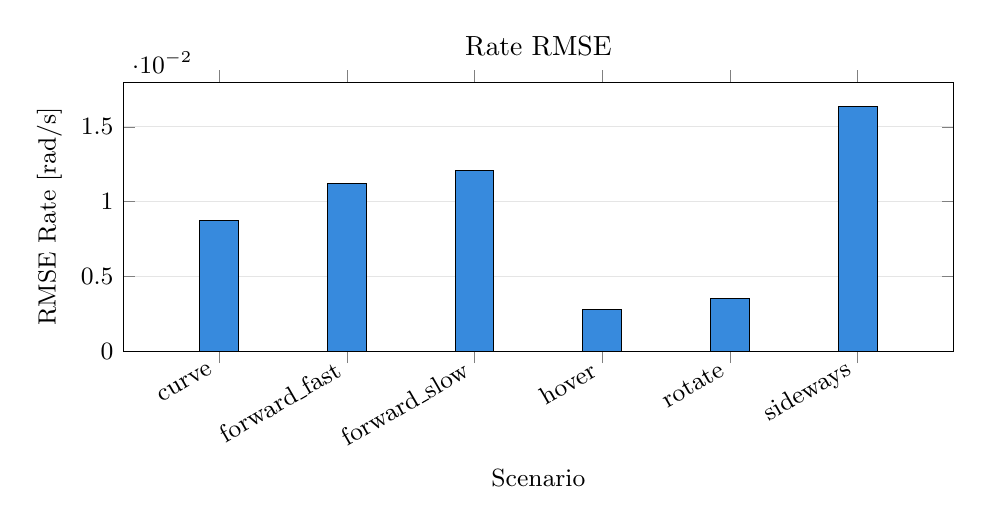
\begin{tikzpicture}
			\begin{axis}[rmse bar, title={Rate RMSE}, ylabel={RMSE Rate [rad/s]}]
				\addplot[fill=barblue] coordinates {
					(curve,0.00876)(forward\_fast,0.01123)(forward\_slow,0.01206)
					(hover,0.00281)(rotate,0.00356)(sideways,0.01635)
				};
			\end{axis}
		\end{tikzpicture}
	\end{subfigure}
	
	\caption{Grouped RMSE (position, velocity, attitude, and angular rate) for the NDI controller with Robust gains across all evaluated flight scenarios.}
	\label{fig:ndi_robust_grouped_rmse}
\end{figure}

\todo{address the hovering problem, as V = 0.}
\todo{one more plot showin that for W20 = 0 only hovering is bad}

Zusammenhang zwischen schlechter windschätzung und schlechter performance im hover mode gerstellen (besonders für NDI)

\begin{table}[htbp]
	\centering
	\caption{Average normalized RMSE per controller/gain combination, averaged across all flight scenarios and state variables.}
	\label{tab:avg_norm_rmse_combo}
	\begin{tabular}{llc}
		\toprule
		Method & Gains & Avg.\ norm.\ RMSE \\
		\midrule
		NDI & Robust & 0.8309 \\
		DFF & Aggressive & 0.9012 \\
		NDI & Aggressive & 1.0278 \\
		DFF & Robust & 1.0320 \\
		DFF & Comp & 1.0405 \\
		PID & Robust & 1.0643 \\
		NDI & Comp & 1.1033 \\
		\bottomrule
	\end{tabular}
\end{table}


The wind compensation is heavily dependant on the quality of the wind estimation.

Setting:

Results
We are looking for one controller which yields the best results for all scenarios. Although we may find better settings for single scenarios we do not want to need to switch.

While theoretically the compensation should allow for a more aggressive PID as the disturbance should compensate the wind disturbance this does not hold up in the results presented. Reason therefore is errors in wind estimation, convergence rates of the KF, maybe even delay of one time step, general uncertainty in the model (uncertain forces etc)

Tuning: The PID controller is retuned on the undisturbed model, as the compensation should eliminate those, allowing for a faster PID control. 
It shows that the retuned PID is far too aggressive and not able to achieve good performance for all flight envelopes, although performing better on some. The reason for this is that although theoretically the Compensation should compensate for the wind, it is not able to fully cancel it due to uncertainties in the wind estimation and state measurements. Hence a robust controller is desired anyways. A combination of the robust PID with the compensation is beneficial. 

Why are the Comp controllers performing bad? -> give examples when they are instable while the others are not. And state that this is the reason why they are not considered in the future.

\subsection{Problems with Observability}
Due to the lack of sensory equipment to measure airspeed the wind estimation depends heavily on the effect of the aerodynamic forces on the airship to estimate the wind velocities. Because only the aerodynamic Forces are directly dependent on the airspeed and thus on the wind velocity. The Compensation uses the current wind estimate to compute the estimation and thus requires a good estimation of wind. Exactly there lies the problem, if the compensation fully compensates for the effect of wind on the airship, the wind estimation quality automatically decreases, leading to a poor estimation and so on. 
To break up this cycle we need to guarantee that the information about the effect of the wind is not fully lost. To achieve this a gain, manipulating the output of the compensation is introduced. This gain in range 0 to 1 determines how aggressively the wind compensation works and balances the wind compensation with the wind estimation.   



\section{Flight Test}